%% Filename: path_filldraw@tikz_for_teachers.tex
%% This code is part of LaTeX with Vim.
%% 
%% Description: TikZ for teachers is free book about TikZ and Sage.
%% 
%% Created: 30.03.12 08:09:17 PM
%% Last Change: 30.03.12 08:09:21 PM
%% 
%% Author: Raniere Gaia Costa da Silva, r.gaia.cs@gmail.com
%% Organization:  
%% 
%% Copyright (c) 2010, 2011, 2012, Raniere Gaia Costa da Silva. All rights 
%% reserved.
%% 
%% This file is license under the terms of a Creative Commons Attribution 
%% 3.0 Unported License, or (at your option) any later version. More details
%% at <http://creativecommons.org/licenses/by/3.0/>.
%

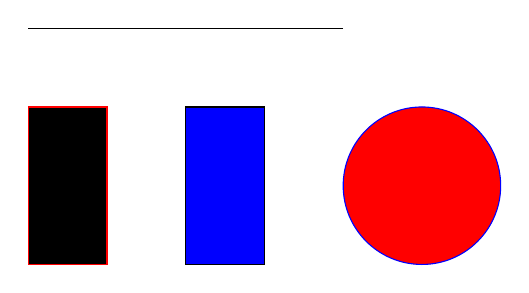
\begin{tikzpicture}
    \path[fill,draw] (0,0) -- (4,0);
    \path[fill,draw=red] (0,-1) rectangle (1,-3);
    \path[fill=blue,draw] (2,-1) rectangle (3,-3);
    \path[fill=red,draw=blue] (5,-2) circle (1);
\end{tikzpicture}
